% ------------------------------------------------------------------------------
% TYPO3 Version 10.4 - What's New (French Version)
%
% @license	Creative Commons BY-NC-SA 3.0
% @link		https://typo3.org/help/documentation/whats-new/
% @language	French
% ------------------------------------------------------------------------------

\section{Changements pour les intégrateurs}
\begin{frame}[fragile]
	\frametitle{Changements pour les intégrateurs}

	\begin{center}\huge{Chapitre 2~:}\end{center}
	\begin{center}\huge{\color{typo3darkgrey}\textbf{Changements pour les intégrateurs}}\end{center}

\end{frame}

% ------------------------------------------------------------------------------
% Feature | 89513 | Provide password recovery for backend users

\begin{frame}[fragile]
	\frametitle{Changements pour les intégrateurs}
	\framesubtitle{Message de récupération de mot de passe (1)}

	\begin{itemize}

		\item Les liens de réinitialisation de mots de passe ne sont valides que pour 4 heures.\newline
			Cette limite n'est pas configurable.
		\item La fonction est désactivable pour tous les utilisateurs ou seulement les administrateurs pour renforcer la sécurité.
		\item Si des utilisateurs partagent une adresse, un texte alternatif de message est utilisé.
		\item Le champ TCA \texttt{be\_users.email} ne doit pas avoir \texttt{eval=email} de défini.

		\item La fonction ne s'applique que pour les utilisateurs qui~:
			\begin{itemize}
				\item ont une adresse email de définie,
				\item ont un mot de passe de défini, et
				\item ne sont pas désactivé/supprimé.
			\end{itemize}

	\end{itemize}

\end{frame}

% ------------------------------------------------------------------------------
% Feature | 89513 | Provide password recovery for backend users

\begin{frame}[fragile]
	\frametitle{Changements pour les intégrateurs}
	\framesubtitle{Message de récupération de mot de passe (2)}

	\begin{itemize}
		\item Il est aussi possible de déclencher la récupération depuis la ligne de commandes.
	\end{itemize}

	\begin{figure}
		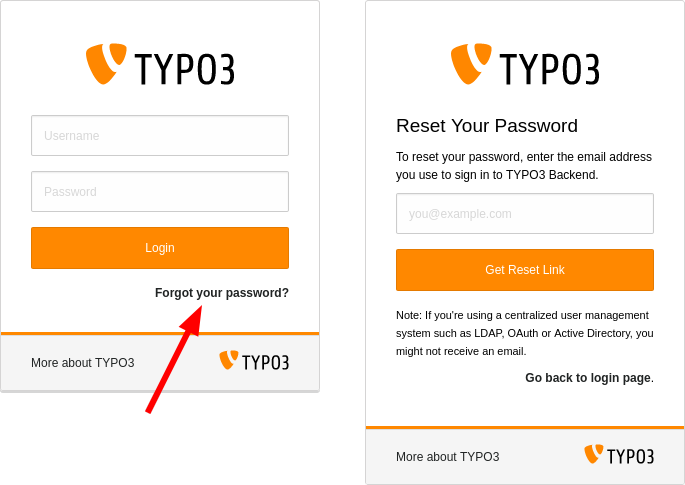
\includegraphics[width=0.9\linewidth]{ChangesForIntegrators/89513-ProvidePasswordRecoveryForBackendUsers.png}
	\end{figure}

\end{frame}

% ------------------------------------------------------------------------------
% Important | 90285 | Fresh installs without constraint for typo3fluid/fluid will get version 3.0+

\begin{frame}[fragile]
	\frametitle{Changements pour les intégrateurs}
	\framesubtitle{Moteur de gabarits Fluid}

	\begin{itemize}
		\item Le noyau de TYPO3 est entièrement compatible avec Fluid version 2.6+ et 3.0+
		\item Les nouvelles installations sans dépendance définie téléchargeront et installeront
			la version 3.x de Fluid (\texttt{typo3fluid/fluid:\^{}3}).
		\item Si votre projet contient des gabarits Fluid incompatibles avec les versions 3.0+,
			effectuez l'une de ces actions~:

			\begin{itemize}
				\item Limiter la version maximale~: \texttt{typo3fluid/fluid:\^{}2}
				\item Mettre à jour les gabarits Fluid.
			\end{itemize}

	\end{itemize}

\end{frame}

% ------------------------------------------------------------------------------
% Important | 18079 | pages.doktype restriction for frontend queries refined

\begin{frame}[fragile]
	\frametitle{Changements pour les intégrateurs}
	\framesubtitle{Gestion du type de page}

	\begin{itemize}
		\item La gestion interne de TYPO3 des types de page a changé.
		\item L'option \texttt{pages.doktype} définie une valeur numérique qui représente le type,
			i.e. page standard, dossier, raccourci, lien vers une url externe, etc.
		\item Les pages de certains types (i.e. dossier et corbeille) étaient exclus lorsque le contenu
			était lut depuis une page ou lors de la récupération d'enregistrements.
		\item Cette limitation est retirée et les types de valeur supérieure à 200 sont possibles.
		\item Il est conseillé aux intégrateurs et développeurs qui utilisent ces types, en TypoScript par exemple,
			de vérifier si le comportement précédent n'était pas abusé et si une mise à jour est nécessaire.
	\end{itemize}

\end{frame}

% ------------------------------------------------------------------------------
% Feature | 90826 | Compare backend usergroups

\begin{frame}[fragile]
	\frametitle{Changements pour les intégrateurs}
	\framesubtitle{Module utilisateur backend}

	\begin{itemize}
		\item Les intégrateurs peuvent désormais comparer des groupes d'utilisateurs backend entre eux.
	\end{itemize}

	\begin{figure}
		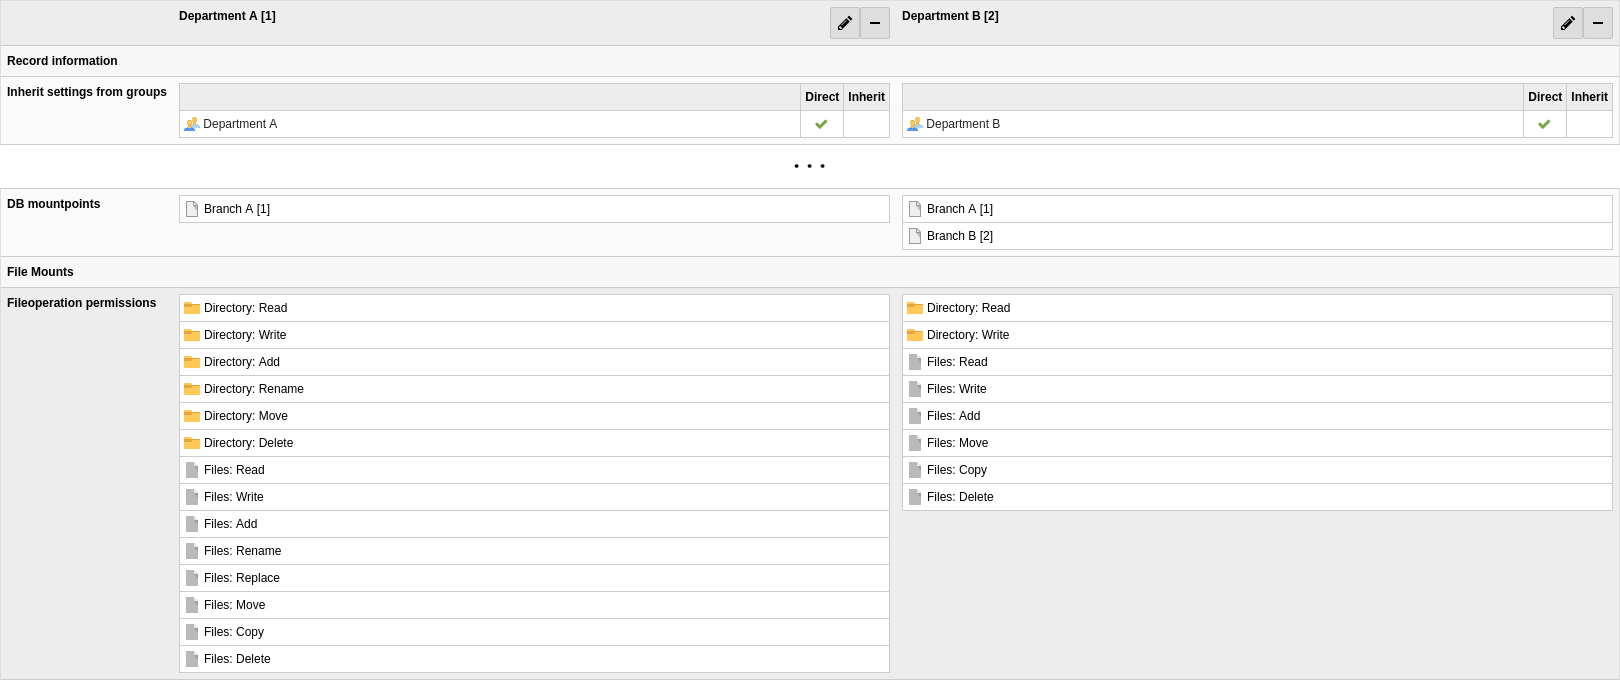
\includegraphics[width=0.9\linewidth]{ChangesForIntegrators/90826-CompareBackendUsergroups.png}
	\end{figure}

\end{frame}

% ------------------------------------------------------------------------------
% Important | 89555 | Workspace-related database records contain the proper Page ID

\begin{frame}[fragile]
	\frametitle{Changements pour les intégrateurs}
	\framesubtitle{Espaces de travail}

	\begin{itemize}
		\item Depuis longtemps, le noyau de TYPO3 définissait le \texttt{pid} à \texttt{-1} pour les enregistrements non publiés.
		\item Les enregistrements versionnés sont maintenant géré par la validation de ces trois champs~:

			\begin{itemize}
				\item \texttt{t3ver\_wsid} (l'ID de l'espace de travail de lequel l'enregistrement est versionné)
				\item \texttt{t3ver\_state} (le type de l'enregistrement versionné)
				\item \texttt{t3ver\_oid} (l'identifiant de l'enregistrement publié)
			\end{itemize}

		\item Ainsi, \texttt{pid=-1} n'est plus nécessaire.
		\item L'assistant de mise à jour converti l'ensemble des champs \texttt{pid} des enregistrements versionnés
			vers leur valeur de \texttt{pid} réelle.
		\item Les nouvelles installations ne sont pas affectées.

	\end{itemize}

\end{frame}

% ------------------------------------------------------------------------------
% Deprecation | 91030 | Runtime-Activated Packages

\begin{frame}[fragile]
	\frametitle{Changements pour les intégrateurs}
	\framesubtitle{Paquets activé à l'exécution}

	\begin{itemize}
		\item La configuration globale suivante est marquée \textbf{dépréciée}~:\newline
			\smaller
				\texttt{\$GLOBALS['TYPO3\_CONF\_VARS']['EXT']['runtimeActivatedPackages']}
			\normalsize
		\item L'usage des extensions activées à l'exécution ralenti considérablement le système.
		\item Il est conseillé aux intégrateurs de mettre en place les corrections nécessaire si un tel avertissement
			est reporté dans le journal de dépréciation~:\newline
			\begingroup
				\fontsize{8}{10}
				\texttt{Support for runtime activated packages will be removed in TYPO3 v11.0.}
			\endgroup

	\end{itemize}

\end{frame}

% ------------------------------------------------------------------------------
